\chapter{Analisis}
\label{chap:analisis}
Pada bab ini dijelaskan mengenai deskripsi perangkat lunak, analisis data histori KIRI, analisis perangkat lunak, dan analisis \textit{heat map}, dan \textit{marker clustering} menggunakan  \textit{Google Maps Javascript API}.


\section{Analisis Data Histori KIRI}
\label{sec:analisisDataHistoriKiri}
Perangkat lunak  akan menggunakan data histori KIRI sebagai sumber data untuk melakukan visualisasi data. Data histori KIRI memiliki format \textit{csv}. Data histori KIRI memiliki lima atribut yaitu:
\begin{itemize}
    \item LogId    sebagai penanda satu record didalam data histori KIRI.
    \item APIKey
    sebagai  atribut api key yang digunakan ketika melakukan perintah pada perangkat lunak KIRI.
    \item Timestamp (UTC)
    atribut untuk mencatat waktu perintah dilakukan format berbentuk \textit{timestamp}.
    \item Action
    jenis action yang dilakukan user pada saat menggunakan perangkat lunak KIRI. Terdapat empat nilai action pada data histori KIRI yakni:
    \begin{itemize}
        \item \textit{PAGELOAD}.
        \item \textit{SEARCHPLACE}.
        \item \textit{WIDGETLOAD}.
        \item \textit{FINDROUTE}.
    \end{itemize}
    \item AdditionalData atribut yang digunakan untuk mencatat informasi tambahan berdasarkan action yang dipilih. Nilai pada additionaldata akan bergantung pada action yang dipilih:
    \begin{itemize}
        \item Jika action bernilai \textit{PAGELOAD} maka additionaldata akan bernilai ip dari pengakses.
        \item Jika action bernilai \textit{SEARCHPLACE} maka additionaldata akan bernlai keyword yang dituliskan oleh pengakses.
        \item Jika action bernilai \textit{FINDROUTE} maka additionaldata akan bernilai posisi tempat dan tujuan dalam bentuk langtitude dan longtitude  yang dicari oleh pengakses.
        \item Jika action bernilai \textit{WIDGETLOAD} maka additionaldata akan bernilai alamat url dari penyedia widget.
    \end{itemize}
\end{itemize}



% \section{Analisis Google Maps Javascript API}
% Perangkat lunak yang akan menggunakan \textit{google maps javascript api} untuk dapat melakukan visualisasi data kedalam bentuk \textit{heatmap} dan \textit{marker clustering}. Untuk dapat menampilkan \textit{map} dan menggunakan fitur yang disediakan oleh \textit{Google Maps Javascript API} maka objek \textit{map} perlu dinisialisaikan. 



\section{Deskripsi Perangkat Lunak}
\label{sec:deskripsiPL}
Pada skripsi ini akan dibangun aplikasi yang bertujuan untuk menemukan pola dengan tool visualisasi. Aplikasi ini akan menggunakan data histori perangkat lunak KIRI sebagai sumber data. Aplikasi ini akan dibangun menggunakan \textit{tools} nodejs dan akan mengimplementasikan \textit{google maps javascript api} sebagai tool untuk melakukan visualisasi data. Beberapa fitur yang dirancang dalam perangkat lunak ini:
\begin{itemize}
\item Perangkat lunak dapat memfilter data berdasarkan atribut \textit{start/finish}.
\item Perangkat lunak dapat memfilter data berdasarkan atribut waktu.
\item Perangkat lunak dapat memfilter data berdasarkan atribut hari.
\item Perangkat lunak dapat menampilkan data dalam bentuk \textit{heat map}
\item Perangkat lunak dapat menampilkan data dalam bentuk \textit{marker clustering}.
\end{itemize}
Perangkat lunak ini akan melukan filter data dan memproses data histori kiri dan akan menampilkan data tersebut kedalam bentuk \textit{heat map} dan \textit{marker clustering} untuk mendapatkan pola-pola tertentu berdasarkan data histori tersebut. Gambaran tentang alur komunikasi perangkat lunak dapat dilihat pada gambar \ref{fig:alurKomunikasi}

\begin{figure}[H]
	\centering  
	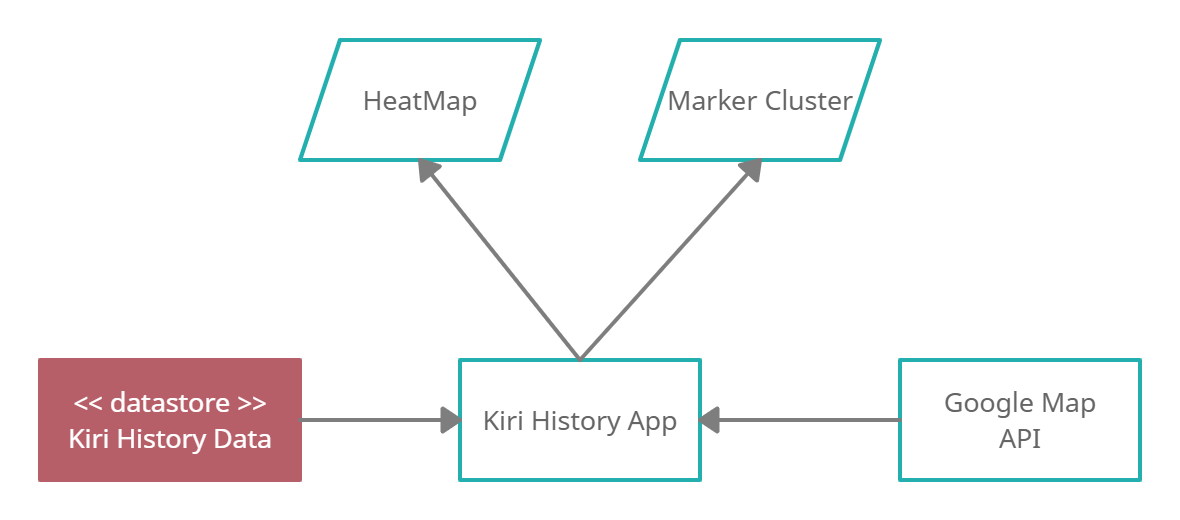
\includegraphics[scale=0.55]{Gambar/software-flow.PNG}  
	\caption[Alur Komunikasi]{Alur Komunikasi} 
	\label{fig:alurKomunikasi} 
\end{figure} 

\begin{enumerate}
\item Perangkat lunak akan mengolah data histori kiri sesuai dengan input yang diberikan.
\item Data yang sudah diolah  akan diubah kedalam format \textit{JSON}.
\item Data yang sudah diolah akan digunakan oleh \textit{Google Maps Javascript API} untuk dapat dilakukan visualisasi data.
\item Perangkat lunak akan memvisualisasikan data kedalam bentuk \textit{heat map} dan \textit{marker clustering}.

\end{enumerate}


\section{Analisis Perangkat Lunak}
Pada subbab ini akan dilakukan analisis untuk aplikasi visualisasi data histori KIRI.
\subsection{Analisis Kebutuhan Perangkat Lunak}
\label{sec:analisisKebutuhanPerangkatLunak}
Berdasarkan latar belakang, rumusan masalah, dan tujuan maka dapat didefinisikan kebutuhan - kebutuhan perangkat lunak visualisasi data histori KIRI sebagi berikut:
\begin{itemize}
    \item Data histori KIRI
    Aplikasi dapat melakukan proses filter pada data histori dan menggunakan data histori KIRI untuk dapat divisualisasikan oleh karena itu diperlukan raw data histori KIRI.
    
    \item Google Maps Javascript API
    Aplikasi dapat melakukan visualisasi data menggunakan \textit{heat map} dan \textit{marker clustering} yang merupakan fitur dari \textit{google maps javascript api}.
    
\end{itemize}
\subsection{Use Case Diagram}
Interaksi antara pengguna dengan perangkat lunak yang dibangun pada skripsi ini digambarkan pada diagram \textit{use case}  \ref{fig:usecase}
\begin{figure}[H]
	\centering  
	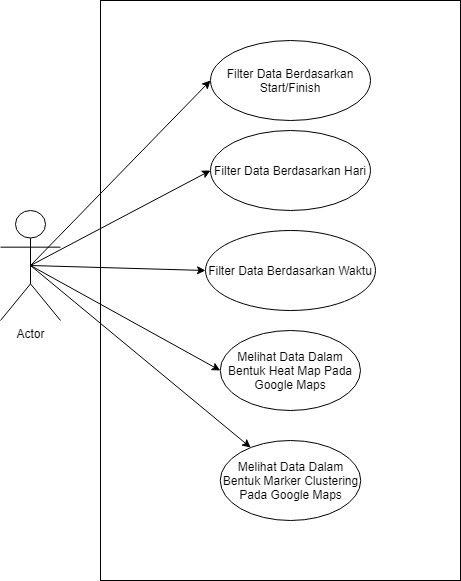
\includegraphics[scale=0.8]{Gambar/KIRI USECASE.jpeg}  
	\caption[Use Case Diagram]{Use Case Diagram} 
	\label{fig:usecase} 
\end{figure} 
\subsection{Use Case Skenario}
Setiap fungsi yang ada pada diagram \textit{use case} dijelaskan dengan skenario untuk memberi gambaran interaksi pengguna dengan sistem.
\begin{table}[H]
    \centering
    \caption{Tabel Skenario Memfilter Data }
    \begin{tabular}{|p{3cm}|p{10cm}|}
    \hline
        Nama & Memfilter Data .\\
    \hline
    \hline
        Deskripsi & Melakukan filter data berdasarkan kategori dari data histori kiri \\
    \hline
        Aktor & Pengguna \\
    \hline
        Pre-kondisi & Aplikasi sudah dijalankan dan sudah dapat mengolah raw data histori KIRI.\\
    \hline
        Alur Skenario Utama & 
        \begin{enumerate}
            \item Sistem memuat aplikasi.
            \item Sistem menampilkan data.
            \item Pengguna  dapat memfilter data berdasarkan waktu,hari, dan \textit{start / finish}.
            \item Sistem melakukan proses filtering berdasarkan atribut yang telah dipilih pengguna.
        \end{enumerate}\\
    \hline
    \end{tabular}
    \label{tab:skenario1}
\end{table}


\begin{table}[H]
    \centering
    \caption{Tabel Skenario Melihat Visualisasi Data Pada Map }
    \begin{tabular}{|p{3cm}|p{10cm}|}
    \hline
        Nama & Melihat Visualisasi Data Pada Map.\\
    \hline
    \hline
        Deskripsi & Melihat hasil visualisasi data pada google map  \\
    \hline
        Aktor & Pengguna \\
    \hline
        Pre-kondisi & Aplikasi sudah dijalankan dan sudah dapat menampilkan data histori KIRI.\\
    \hline
        Alur Skenario Utama & 
        \begin{enumerate}
            \item Sistem menampilkan data yang telah difilter oleh pengguna.
             \item Pengguna  dapat memilih akan menggunakan metode visulasisai \textit{heat map} atau \textit{marker clustering}.
            \item Sistem menampilkan hasil visualisasi data berdasarkan metode yang telah dipilih pengguna.
        \end{enumerate}\\
    \hline
    \end{tabular}
    \label{tab:skenario1}
\end{table}

\subsection{Data Flow Diagram}
Interaksi data dalam perangkat lunak yang dibangun pada skripsi ini digambarkan pada \textit{data flow diagram} \ref{fig:dfd_0}
\begin{figure}[H]
	\centering  
	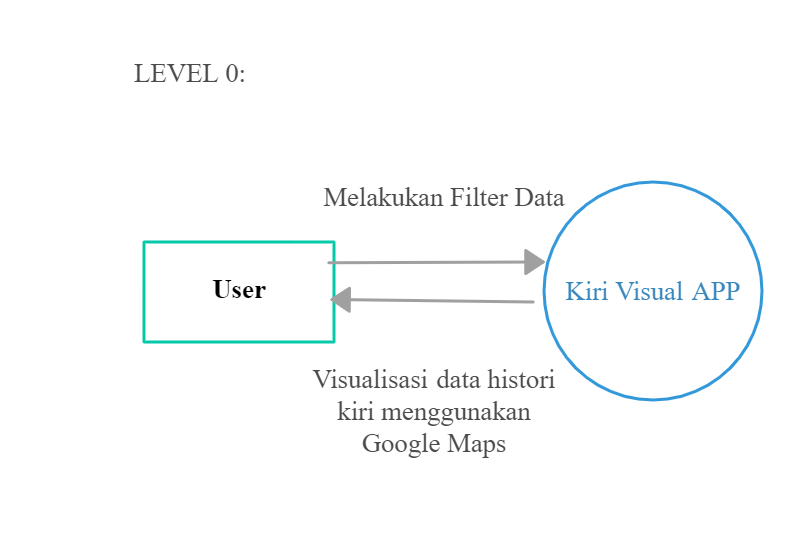
\includegraphics[scale=0.4]{Gambar/DFD_0.png}  
	\caption[Data Flow Diagram Level 0]{Data Flow Diagram Level 0} 
	\label{fig:dfd_0} 
\end{figure} 

Pada level 0 ini dapat dilihat pada gambar \ref{fig:dfd_0}, perangkat lunak yang akan dibuat memiliki dua buah flow utama yaitu user dapat melakukan penyaringan data, dan user dapat menerima hasil penyaringan data dalam bentuk visualisasi pada \textit{google maps}. Setelah dilakukan pengujian lebih lanjut maka didapatkan \textit{data flow diagram level 1} \ref{fig:dfd_1}

\begin{figure}[H]
	\centering  
	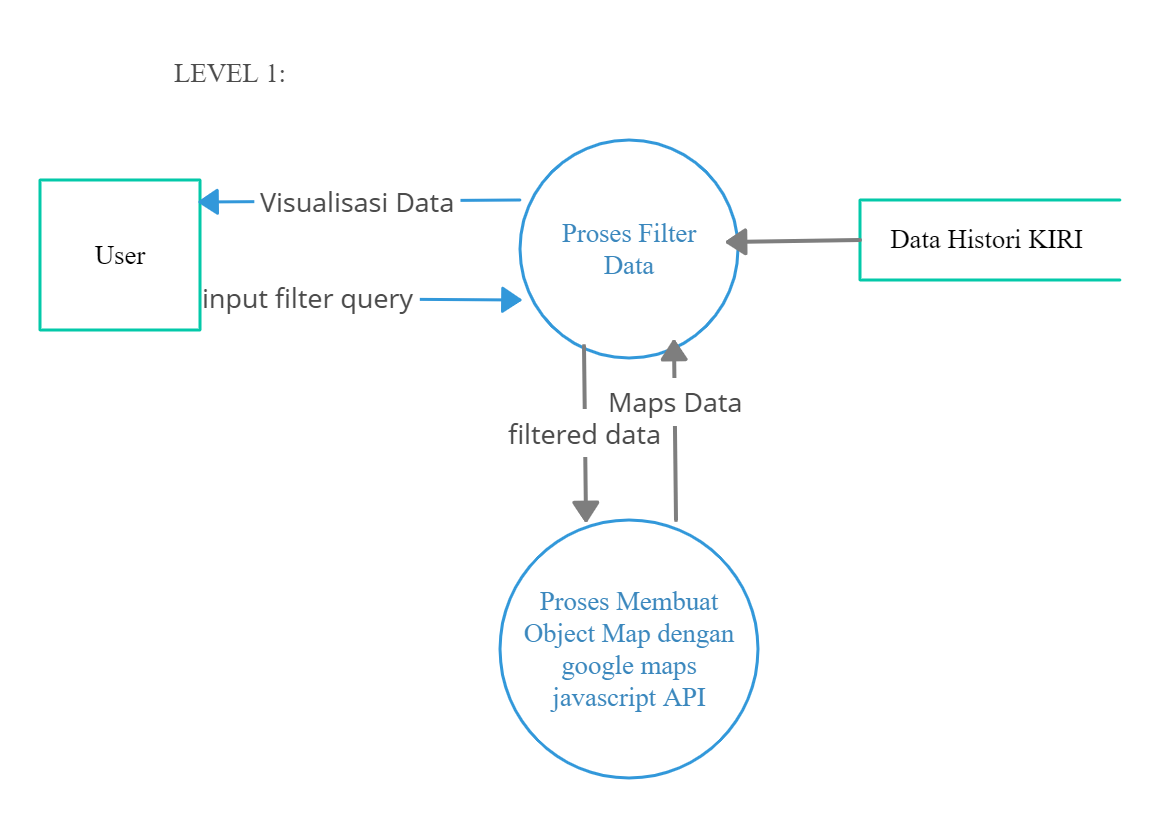
\includegraphics[scale=0.3]{Gambar/DFD_1.png}  
	\caption[Data Flow Diagram Level 1]{Data Flow Diagram Level 1} 
	\label{fig:dfd_1} 
\end{figure} 

Pada level 1 ini dapat dilihat pada gambar \ref{fig:dfd_1}, perangkat lunak akan memiliki dua buah proses utama yaitu:
\begin{itemize}
    \item Filter data proses untuk melakukan penyaringan data histori kiri berdasarkan \textit{query input} dari user.
    \item Proses pembuatan object \textit{maps} proses yang akan menerima data histori KIRI dan membuat objek map menggunakan \textit{google maps javascript api}.
\end{itemize}

Berdasarkan \textit{data flow diagram } pada gambar \ref{fig:dfd_1}, pada perangkat lunak yang akan dibuat user dapat melakukan tiga buah aksi:

\begin{enumerate}
  \item Filter data histori KIRI user dapat memasukan filter parameter untuk melakukan proses penyaringan data histori KIRI, dan perangkat lunak akan melakukan proses penyaringan berdasarkan filter parameter yang dipilih user.
  \item Select mode visualisasi user dapat memilih mode visualisasi pada perangkat lunak ini, akan disediakan dua mode visualisasi \textit{heatmap} dan \textit{marker clustering}.
  \item Visualisasi data dengan google maps pada perangkat ini user akan menerima output berupa data yang telah tervisualisasi dengan google map.
\end{enumerate}

\subsection{Flow Chart Diagram}
Alur perangkat lunak yang akan dibuat dapat digambarkan kedalam bentuk \textit{flow chart}  \ref{fig:fc}
\begin{figure}[H]
	\centering  
	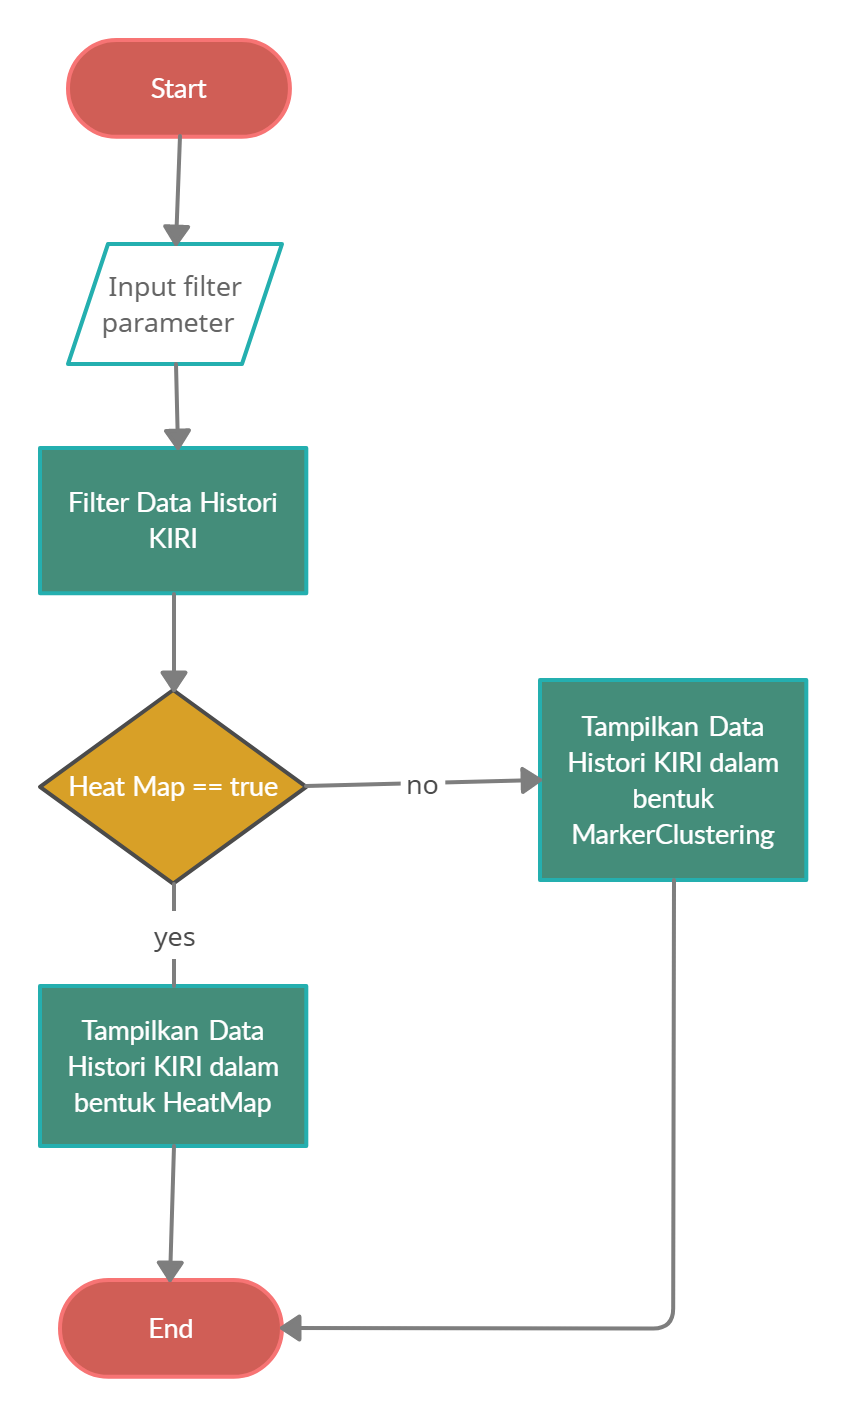
\includegraphics[scale=0.3]{Gambar/KIRI_Flow_Chart.png}  
	\caption[KIRI Flow Chart]{KIRI Flow Chart} 
	\label{fig:fc} 
\end{figure} 


\subsection{Input dan Output}
Input dan output yang akan diterima oleh perangkat lunak yang akan dibuat adalah sebagai berikut.

\begin{itemize}
    \item Input Filter Parameter filter parameter adalah semua parameter yang  dapat dipilih user untuk dapat melakukan penyaringan data histori KIRI, pada perangkat lunak yang akan dibangun user dapat memilih tiga filter parameter.
    
    \item Input mode visualisasi pada perangkat lunak yang akan dibangun user dapat memilih dua mode visualisasi yaitu \textit{mode heatmap} dan \textit{mode markerclustering}.
    
    \item Output visualisasi data output pada perangkat lunak yang akan dibangun adalah hasil visualisasi data histori KIRI dalam bentuk \textit{marker clustering} atau bentuk \textit{heat map}.
\end{itemize}